\documentclass[12pt]{report}
% English hyphenation
\usepackage[british]{babel}
% Links
\usepackage[breaklinks=true]{hyperref}
% Images
\usepackage{graphicx}
\graphicspath{ {./images/} }

\usepackage[noabbrev]{cleveref}

\crefname{appsec}{Appendix}{Appendices}

\usepackage[utf8]{inputenc}
\usepackage{csquotes}

\usepackage{caption}
\usepackage{subcaption}
\usepackage[a4paper, headheight=15pt]{geometry}

\usepackage[load-configurations=abbreviations, binary-units=true]{siunitx}

\usepackage{fancyhdr}
\pagestyle{fancy}
\fancyhead{}
\fancyhead[L]{\leftmark}
\fancyhead[R]{\rightmark}
\fancyfoot{}
\fancyfoot[C]{\thepage}
\renewcommand{\headrulewidth}{0.4pt}
\renewcommand{\footrulewidth}{0.4pt}
\renewcommand{\chaptermark}[1]{ \markboth{#1}{} }
\renewcommand{\sectionmark}[1]{ \markright{#1}{} }


\newcommand{\imagesource}[1] {\caption*{\begin{footnotesize} Source: \url{#1} \end{footnotesize}}}
% Appendix
\usepackage[toc,page]{appendix}
% Change name of toc
\renewcommand*\contentsname{Table of Contents}

\usepackage[style=numeric,sorting=none]{biblatex}
\addbibresource{bibliography.bib}

\title{Shape Tracking Spiking Neural Network}
\author{Filippo Ferrari}
\date{April 2019}


\begin{document}

\begin{titlepage}
	\newcommand{\HRule}{\rule{\linewidth}{0.5mm}} % Defines a new command for horizontal lines, change thickness here
	
	\center % Centre everything on the page
	
	%------------------------------------------------
	%	Headings
	%------------------------------------------------
	
	\textsc{\LARGE University of Manchester}\\[1cm] % Main heading such as the name of your university/college
	
	\textsc{\Large School of Computer Science}\\[1.5cm] % Major heading such as course name
	
	
	%------------------------------------------------
	%	Title
	%------------------------------------------------
	
	\HRule\\[0.4cm]
	
	{\huge\bfseries Shape Tracking\\
	Spiking Neural Network}\\[0.4cm] % Title of your document
	
	\HRule\\[2.0cm]
	
	%------------------------------------------------
	%	Author(s)
	%------------------------------------------------
	
	\begin{minipage}{0.4\textwidth}
		\begin{flushleft}
			\large
			\textit{Author}\\
			Filippo \textsc{Ferrari} % Your name
		\end{flushleft}
	\end{minipage}
	~
	\begin{minipage}{0.4\textwidth}
		\begin{flushright}
			\large
			\textit{Supervisor}\\
			Prof. Steve \textsc{Furber} % Supervisor's name
		\end{flushright}
	\end{minipage}
	
    \vfill\vfill
    
	\textsc{\large BSc Artificial Intelligence\\
	with Industrial Experience}\\[0.5cm] % Minor heading such as course title

	%------------------------------------------------
	%	Date
	%------------------------------------------------
	
	\vfill\vfill\vfill % Position the date 3/4 down the remaining page
	
	{\large April 2019} % Date, change the \today to a set date if you want to be precise

\end{titlepage}

\thispagestyle{plain}
\chapter*{Abstract}
This report will present a biologically inspired spiking neural network which can be used to recognise and track simple shapes moving in a video stream in real time. The network presented runs in biological real time on a 4 chips SpiNNaker board, a massively-parallel multi-core computing system. 

The first chapter will briefly introduce the functioning of biological neurons and the technologies used in order to simulate them: the aforementioned SpiNNaker system, Dynamic Vision Sensors, and a software emulator to emulate these with common frame-based devices.

The second chapter will first introduce PyNN, an high level language based on Python used to implement spiking neural networks and generate SpiNNaker compatible executables, and then will describe in detail the architecture of network and the links between the network and neurobiology.

In the third chapter the approach to code testing and a discussion on the problem on how to evaluate the network performance will be presented. Correctly evaluating this spiking neural network posed several problems and a proper way to evaluating it has not been found.

The last chapter will focus on reflections on the planning and management of this project together with the challenges faced. 


\chapter*{Acknowledgements}
Firstly, I would like to thank my supervisor, Prof.\ Steve Furber for agreeing to supervise this project and for all the help and guidance he offered throughout the past year. 

I would like to thank Petruț Bogdan, who pointed me towards useful resources and took time to discuss them with me, and Dr.\ Garibaldi Pineda Garcia for his very great DVS emulator. Also, I am deeply grateful to Andrew Rowley for his help in setting up the SpiNNaker development environment. 

I am extremely grateful to Matt, Rob and the entire Research team of Innovative Technology for arranging for me to work with them after my placement and for all the things I have learnt in the past two years.

Special thanks go to Giordana, Federica, Michele, Andrea, Sam, Lorenzo, Stefano and Gabriele for helping me and supporting me during the past year. 

I cannot express my gratitude to Costanza for everything she has done for me in the past 4 years. 

Last, but definitely not least, I want to thank my family for their continue support and encouragement.

\tableofcontents

\listoffigures

\listoftables

\chapter{Context}
This project investigates whether biologically inspired spiking neural network can be used to recognise and track shapes in a video stream in real time. 

In this chapter a brief introduction on the functioning of biological neurons and the technologies used in order to simulate them will be presented. A quick discussion on the motivation and previous work in the area will also provided. 

All of the following tools and technologies had been selected in order to develop a project with as many similarities as possible to the functioning of a biological brain. 

\section{Neuron}
Neurons are highly specialised cells found in the nervous system designed to generate and transmit electrical signals to other cells. Many different kinds of neurons exist \cite{Llinas:2008}, each with different morphology, but a typical neuron can be divided in three parts shown in \cref{fig:neuron_morphology} \textbf{A}:
\begin{itemize}
    \item Soma: a usually compact area which represents the body of the neuron and which contains the cell nucleus.
    \item Dendrites: tree-like extensions of the soma membrane which acts as the ``input'' pole to the neuron.
    \item Axons: a cable-like structure that acts as the ``output'' pole of the neuron and propagate neuronal output to other cells.
\end{itemize}
The axon of a \textit{presynaptic cell} makes contact with the dendrite of a \textit{postsynaptic cell} at a site called synapse \cite{Gerstner:2014}, highlighted in \cref{fig:neuron_morphology} \textbf{B}.

\begin{figure}[ht]
\centering
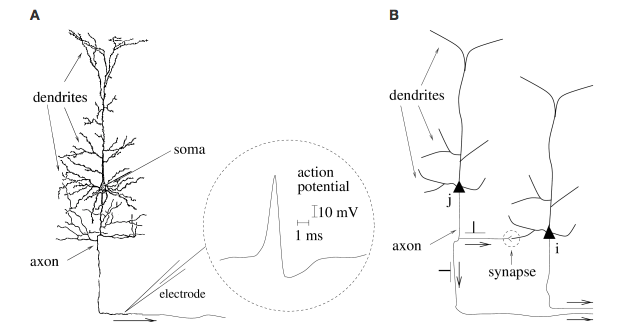
\includegraphics[scale=0.6]{images/neuron.png}
\caption[Neuron Morphology]{\textbf{A}. A cortical pyramidal cell with its soma, axon and dendrites highlighted. \textbf{B}. Signal transmission from neuron $j$ (presynaptic cell) to neuron $i$ (postsynaptic cell). Reproduced from \cite{Gerstner:2014}.}
\label{fig:neuron_morphology}
\end{figure}

A neuron spikes when the current input carried by the dendrites exceeds a certain threshold. The biochemical details of this process are not relevant for this project and the variety in electrophysiological properties of neurons \cite{Llinas:2008} leads to necessary simplification in order to simulate them. The signals emitted by neurons are called action potentials or spikes, and an approximate form is shown in the circled area of  \cref{fig:neuron_morphology}. A key property of action potential is that the form does not carry any information, information is actually carried by the number of action potentials and their timings \cite{Gerstner:2014}. After each spike the neuron enters a state called refractory period, in which it is impossible for it to spike again.  

Several mathematical models are available in order to simulate neurons, the one used in this project is a leaky integrate-and-fire (LIF) neuron model. 

% TODO insert maths details of LIF model

\subsection{Spiking Neural Networks}
Spiking neural networks are artificial neural networks which are closer to biology than the one commonly used nowadays for machine learning tasks. In spiking neural networks the concept of time is introduced and the communication between neurons relies exclusively on discrete spikes, the ones described in the previous section, instead of continuous values. 

The field of spiking neural networks is still in its infancy and lacks an effective supervised method for training, the equivalent of backpropagation for artificial neural network.


\section{SpiNNaker}
In order to handle the obvious complexity of neural simulation two approaches are possible. The first one is to use supercomputer built for general purpose task like in the case of the Blue Brain project which uses IBM's Blue Gene supercomputers \cite{Markram2006}. The second approach is to employ neuromorphic systems. These systems are designed around the idea that small computing elements (the ``neurons'') perform computation in a highly distributed manner in ways that mimic biological brains \cite{Furber2016}. Several of these systems have been developed recently, for example IBM TrueNorth, Stanford Neurogrid and University of Manchester SpiNNaker, which will be the system used for this project.

SpiNNaker is a massively-parallel multi-core computing system designed for large scale brain simulations running in biological real time. The system had been designed focusing on scalability, in order to model the very large number of components in a biological brain, and energy efficiency.

\begin{figure}[ht]
\centering
\begin{subfigure}{0.45\textwidth}
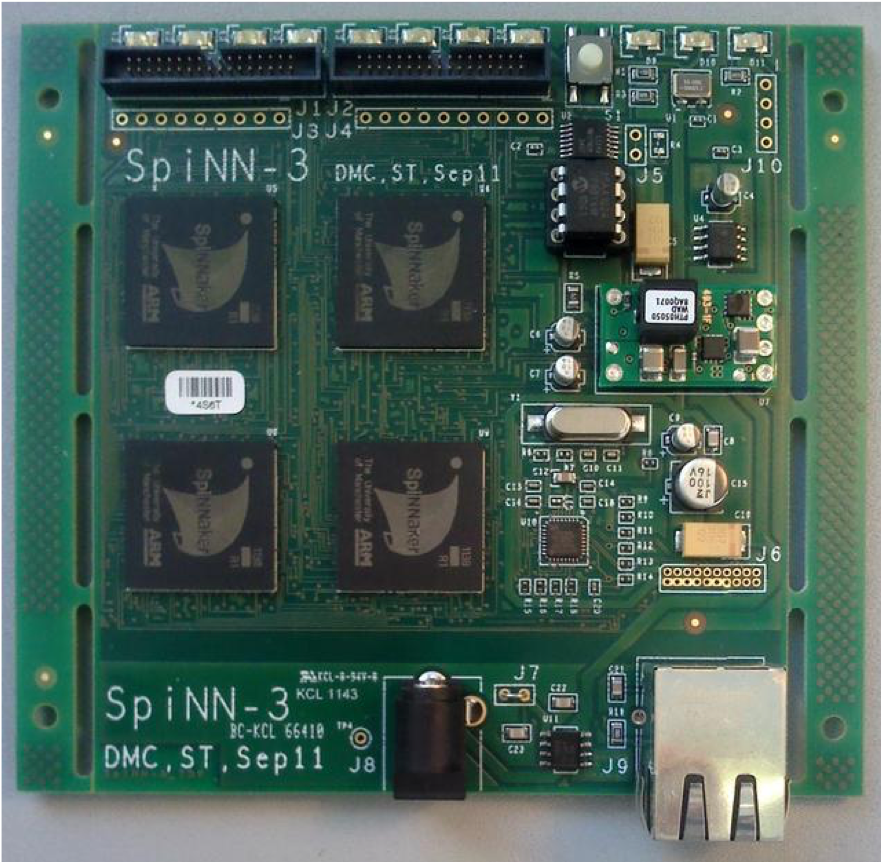
\includegraphics[width=\textwidth]{images/spinnaker_board.png} 
\caption{SpiNNaker board with 4 chips.}
\label{fig:spinnaker_board}
\imagesource{http://apt.cs.manchester.ac.uk/projects/SpiNNaker/hardware/index3.php}
\end{subfigure}
\begin{subfigure}{0.45\textwidth}
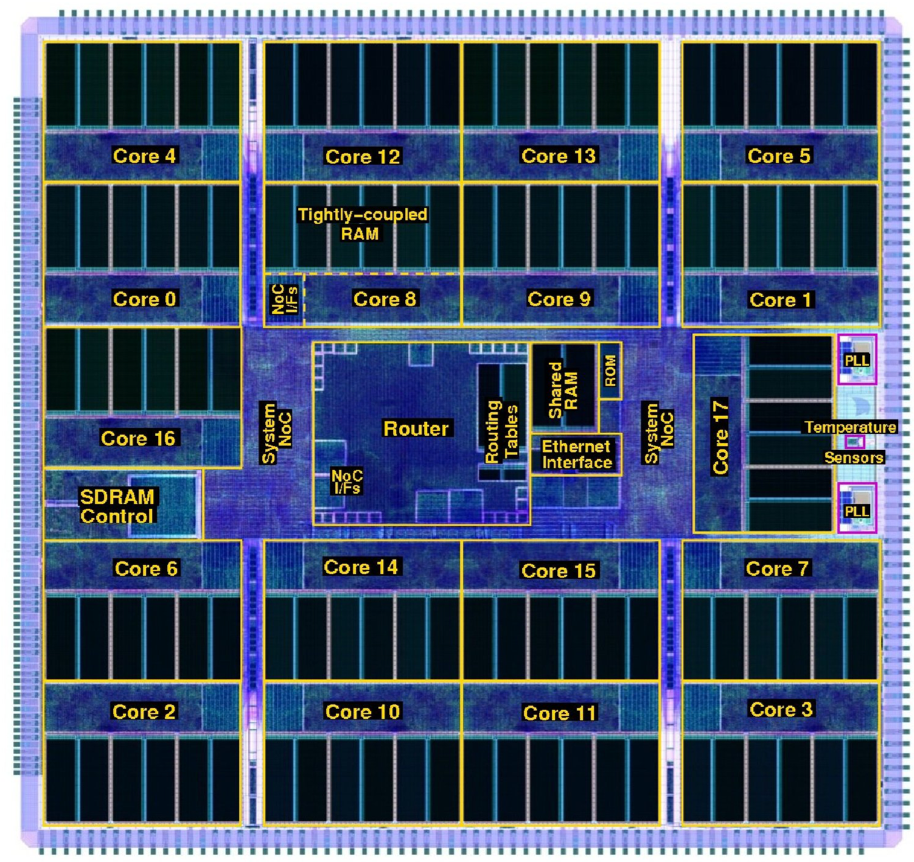
\includegraphics[width=\textwidth]{images/spinnaker_chip.png}
\caption{SpiNNaker chip}
\label{fig:spinnaker_chip}
\imagesource{http://apt.cs.manchester.ac.uk/projects/SpiNNaker/SpiNNchip}
\end{subfigure}
\caption[SpiNNaker Board and Chip]{SpiNNaker board and chip}
\label{fig:spinnaker}
\end{figure}

SpiNNaker is available at different scale, from a 4 chips board shown in \cref{fig:spinnaker_board} to a 1,036,800 cores machine accessible through the Neuromorphic Computing platform of the Human Brain Project \footnote{\url{https://www.humanbrainproject.eu/en/silicon-brains/} --- Accessed 19 April 2019}.

For this project, a 4 chips board has been used. Each chip, \cref{fig:spinnaker_chip} includes 18 ARM9 cores and \SI{128}{\mega\byte} of SDRAM. The board is connected to a host machine through an Ethernet cable and it is powered through a \SI{5}{\volt} \SI{1}{\ampere} USB cable.


\section{Dynamic Vision Sensor}
Due to the biologically inspired nature of this project and of the technologies involved, it made sense to use a Dynamic Vision Sensor as the input to the spiking neural network. A Dynamic Vision Sensor, also known as digital retina, is a device that records relative intensity changes for each individual pixel in continuous time.

\section{Motivation}


\section{Previous Work}


\chapter{Conclusion}
\section{New Knowledge}
The project required learning and understanding a lot of material which is not part of my degree. In particular, learning enough in order to understand the computational neuroscience literature required a great deal of effort and time. The lack of literature related to this specific task for spiking neural network was another obstacle which posed a great chance of failure. 

Luckily, Python was already known and only the PyNN API required to be learnt. 

\section{Project Development}
The project development run for 20 weeks, 12 in Semester 1 and 8 in Semester 2. The project presentation was planned to be between week 6 and 8 of Semester 2, so week 6 had been taken as the deadline for the actual development. Also, development stopped during Christmas for revision.

\begin{table}[ht]
\centering
\begin{tabular}{l|ll}
Milestones                    & Planned Weeks & Actual Weeks \\ \hline
Research                      & 1-4           & 1-6          \\
SpiNNaker Setup               & 1-4           & 1-3          \\
DVS Emulator Setup            & 5-8           & 4-8          \\
Receptive Fields Working      & 8-11          & 8-12         \\
Shapes using Synthetic Videos & 12-15         & 13-16        \\
Shapes using Webcam           & 15-18         & 16-19       
\end{tabular}
\caption{Milestones of the project and planned and actual weeks of development.}
\label{table:development}
\end{table}

\Cref{table:development} shows the main milestones of the project, how the development had been planned in September and how it went during the academic year.

A lot of time had been allocated for research and the initial setup. When devising the original plan, extra time had been added to each milestone. Retrospectively, this had been a good decision as it allowed the project to run pretty much on schedule throughout the year.

The biggest problem faced during the development was caused by an undetected bug in the code which sets the connections between cells populations. Due to this bug, getting the receptive fields to work as expected took longer than expected and added an extra week of development to the original plan. Other reasons causing delays were due to unreported incompatibilities in some of the libraries used during the 

\section{Reflection}
Overall, this project had been a great learning experience spanning different fields. 

Most of the planned milestones had been achieved. In particular, the network runs in real time on a 4 chips SpiNNaker board and achieves sensible results on the synthetic video.

Nevertheless, several limitations are still present. The network cannot be easily expanded in order to recognise new shapes: the connections have to be manually created for each new shape. Also, following the results shown in \cref{fig:shape_webcam_input}, the webcam input is too noisy for being useful. It is opinion of the author that in order to solve this problems, a deeper network, with populations of cells encoding higher levels of abstraction, could be used together with a learning algorithm like Spike Timing Dependent Plasticity (STDP) \cite{Song2000} in order to learn the connection weights between the cells populations. 

\appendix
\chapter{Appendix Title}
Appendix goes here...

%\setcitestyle{numbers}
%\bibliography{bibliography}

\printbibliography

\end{document}
